\section{State of the Art}

In this section, we aim to review four dimensionality reduction techniques that we will later apply our divide-and-conquer framework to. Next, we will showcase in more detail the work of Delicado and Pachón-García with respect to MDS in big data (\cite{Delicado2024}) to motivate our choosing of the divide-and-conquer approach. Finally, we will discuss three more appreciable solutions to the big data problem in DR and how they relate to our proposal: Landmark Isomap (\cite{Silva2002}), the Out-of-Core Dimensionality Reduction Framework (\cite{Reichmann2024}) and formidable Python t-SNE implementations.

\subsection{A few Dimensionality Reduction Techniques}

\subsubsection{Non-classical MDS. The SMACOF algorithm}

SMACOF (Scaling by MAjorizing a COmplicated Function) is a multidimensional scaling algorithm that minimizes metric stress using a majorization technique (\cite{Borg1997}). Also known as the Guttman Transform, this technique is more powerful for this problem than general optimization methods, such as gradient descent.

\begin{algorithm}
    \caption{SMACOF}
    \label{alg:SMACOF}
    
    \begin{algorithmic}[1]
    \REQUIRE $D_{\mathcal{X}} = (\delta_{ij})$, the matrix of observed distances; $q$, the embedding's dimensionality; $n\_iter$, the maximum number of iterations; and $\epsilon$, the convergence threshold.
    \ENSURE $\tilde{\mathcal{Y}}$, a configuration in a $q$-dimensional space.
    \STATE Initialize $\tilde{\mathcal{Y}}^{(0)} \in \mathbb{R}^{n \times q}$
    \STATE $k \leftarrow 0$
    \REPEAT
        \STATE Compute distance matrix of $\tilde{\mathcal{Y}}^{(k)}$:  $d_{ij}(\tilde{\mathcal{Y}}^{(k)}) = \|x_i - x_j\|$
        \STATE Compute the Metric STRESS: $STRESS_M(D_{\mathcal{X}}, \tilde{\mathcal{Y}}^{(k)}) = \sqrt{\frac{\sum_{i<j}\left(\delta_{i j}-d_{i j}\right)^2}{\sum_{i<j} \delta_{i j}^2}}$
        \STATE Compute the Guttman Transform: $\tilde{\mathcal{Y}}^{(k+1)} = n^{-1}B(\tilde{\mathcal{Y}}^{(k)})\tilde{\mathcal{Y}}^{(k)}$ where $B(\tilde{\mathcal{Y}}^{(k)}) = (b_{ij})$:
        $$
        b_{ij} =
        \begin{cases}
        -\delta_{ij}/d_{ij}(\tilde{\mathcal{Y}}^{(k)}) & \text{if } i \neq j \text{ and } d_{ij}(\tilde{\mathcal{Y}}^{(k)}) > 0 \\
        0 & \text{if } i \neq j \text{ and } d_{ij}(\tilde{\mathcal{Y}}^{(k)}) = 0 \\
        -\sum_{j \neq i} b_{ij} & \text{if } i = j
        \end{cases}
        $$
        \STATE $k \leftarrow k + 1$
    \UNTIL{$k \geq n\_iter$ or $|STRESS_M(D_{\mathcal{X}}, \tilde{\mathcal{Y}}^{(k-1)}) - STRESS_M(D_{\mathcal{X}}, \tilde{\mathcal{Y}}^{(k)}| < \epsilon$}
    \RETURN $\tilde{\mathcal{Y}}^{(k)}$
    \end{algorithmic}
\end{algorithm}

\subsubsection{Local MDS}

Local MDS (\cite{Chen2009}) is a variant of non-classical multidimensional scaling that differs in how large distances are treated. Specifically, a repulsive term between distant points is added to the stress function to further separate points in the low-dimensional configuration.

\begin{algorithm}
    \caption{Local MDS}
    \label{alg:LocalMDS}
    
    \begin{algorithmic}[1]
    \REQUIRE $D_{\mathcal{X}}$, the matrix of observed distances; $q$, the embedding's dimensionality; $k$, the size of neighborhoods; and $\tau$, the weight of the repulsive term.
    \ENSURE $\tilde{\mathcal{Y}}$, a configuration in a $q$-dimensional space.
    \STATE Compute the symmetrized k-NN graph of $D_{\mathcal{X}}$, $\mathcal{N}$
    \STATE Calculate $t=\frac{|\mathcal{N}|}{\left|\mathcal{N}^C\right|} \cdot \operatorname{median}_{\mathcal{N}}\left(D_{i, j}\right) \cdot \tau$
    \STATE Minimize $$\sum_{(i, j) \in N}\left(D_{i, j}-\left\|\mathbf{y}_i-\mathbf{y}_j\right\|\right)^2 - t \sum_{(i, j) \notin N}\left\|\mathbf{y}_i-\mathbf{y}_j\right\|$$
    \RETURN The solution to the optimization problem, $\tilde{\mathcal{Y}}$.
    \end{algorithmic}
\end{algorithm}

Parameters $\tau$ (which must be in the unit interval) and $k$ may be tuned with $k'$-cross validation thanks to the LCMC (Local Continuity Meta-Criteria). (\textit{POSSIBLE ANNEX})

\subsubsection{Isomap}

Isomap (\cite{Tenenbaum2000}) is a nonlinear technique that preserves geodesic distances between points in a manifold. The key insight of Isomap is that large distances between objects are estimated from the shorter ones by the shortest path length. Then, shorter and estimated-larger distances have the same importance in a final MDS step.

\begin{algorithm}
    \caption{Isomap}
    \label{alg:Isomap}

    \begin{algorithmic}[1]
    \REQUIRE $D_{\mathcal{X}}$, the matrix of observed distances; $q$, the embedding's dimensionality; and $\epsilon$ or $k$, the bandwidth.
    \ENSURE $\tilde{\mathcal{Y}}$, a configuration in a $q$-dimensional space.
    \STATE Find the $\epsilon$-NN or k-NN graph of $\mathcal{X}$, $G$.
    \STATE Compute the distance matrix of $G$, $D_G$.
    \STATE Embed $D_G$ to a $q$-dimensional space with MDS.
    \RETURN The output configuration of MDS.
    
    \end{algorithmic}
\end{algorithm}

The only tuning parameter of Isomap is the bandwidth ($\epsilon$ or $k$), but there is no consensus on what is the best method to choose it.

\subsubsection{t-SNE}

t-SNE (t-Distributed Stochastic Neighbor Embedding) (\cite{Vandermaaten2008}) is a nonlinear dimensionality reduction technique that preserves local neighborhoods by modeling similarities between points as conditional probabilities. The difference between these probability distributions in high and low-dimensional spaces is then minimized.

\begin{algorithm}
    \caption{t-SNE}
    \label{alg:tSNE}
    
    \begin{algorithmic}[1]
    \REQUIRE $\mathcal{X} \in \mathbb{R}^{n \times p}$, the high-dimensional configuration; $q$, the embedding's dimensionality; perplexity $Perp$.
    \ENSURE $\tilde{\mathcal{Y}}$, a configuration in a $q$-dimensional space.
    \STATE For every datapoint $i$, find $\sigma_i$ so that the conditional probability ditribution
        $$p_{j|i} = \frac{\exp(-\|x_i-x_j\|^2/2\sigma_i^2)}{\sum_{k \neq i}\exp(-\|x_i-x_k\|^2/2\sigma_i^2)}$$ has perplexity $2^{-\sum_{j}p_j \log_2 p_j} = Perp$
    \STATE Symmetrize conditional distributions: $p_{ij} = \frac{p_{j|i} + p_{i|j}}{2n}$ if $i\neq j$, $p_{ii} = 0$
    \STATE Consider Student t-distributed joint probabilities for the low-dimensional data $y_i$: $$q_{ij} = \frac{(1 + \|y_i-y_j\|^2)^{-1}}{\sum_{h \neq k}(1 + \|y_h-y_k\|^2)^{-1}}$$
    \STATE Minimize the sum of Kullback-Leibler divergences between the joint distributions over all datapoints: $$C(\tilde{\mathcal{Y}})=\sum_i \sum_j p_{j \mid i} \log \frac{p_{j \mid i}}{q_{j \mid i}}$$
    \RETURN The solution to the optimization problem, $\tilde{\mathcal{Y}}$.
    
    \end{algorithmic}
\end{algorithm}

t-SNE focuses on retaining the local structure of the data while ensuring that every point $y_i$ in the low-dimensional space will have the same number of neighbors, making it particularly effective for visualizing clusters. The use of the Student t-distribution in the low-dimensional space addresses the \textit{crowding problem} by allowing dissimilar points to be modeled far apart (\cite{Vandermaaten2008}).

Perplexity is interpreted as the average effective number of neighbors of the high-dimensional datapoints $x_i$ and typical values are between 5 and 50.

\subsection{Multidimensional Scaling for Big Data}

\cite{Delicado2024} compared four existing versions of MDS with two newly proposed (Divide-and-conquer MDS and Interpolation MDS) to handle large data. As can be seen in Figure \ref{fig:bigmds}, these can be grouped into four categories:

\begin{itemize}
    \item \textbf{Interpolation-based}: Landmark MDS, Interpolation MDS and Reduced MDS apply classical multidimensional scaling to a subset of $l \ll n$ points and then interpolate the projection of the remaining data. They differ in how the interpolation is computed: Landmark MDS uses distance-based triangulation; Interpolation MDS, the $l$-points Gower Interpolation Formula; and Reduced MDS, the 1-point Gower Interpolation Formula.
    \item \textbf{Approximation-based}: Pivot MDS approximates the SVD of the full inner product matrix with the SVD of the inner product matrix between a subset of $l \ll n$ points and all the points in the dataset.
    \item \textbf{Divide-and-conquer}: In Divide-and-conquer MDS, the dataset is randomly partitioned into subsets of up to $l \ll n$ points into which MDS is independently applied. Then, the resulting embeddings are aligned with Procrustes transformations.
    \item \textbf{Recursive}: Fast MDS is similar in spirit to Divide-and-conquer MDS, but it partitions the data recursively. 
\end{itemize}

\begin{figure}[ht]
    \centering
    \captionsetup[subfigure]{labelformat=empty}

    \begin{subfigure}[t]{0.3\textwidth}
        \centering
        \includegraphics[width=.7\textwidth]{figures/landmark_MDS.png}
        \caption{Landmark MDS}
        \label{fig:landmark_MDS}
    \end{subfigure}
    \hfill
    \begin{subfigure}[t]{0.3\textwidth}
        \centering
        \includegraphics[width=.7\textwidth]{figures/interpolation_adac.png}
        \caption{Interpolation MDS}
        \label{fig:interpolation_MDS}
    \end{subfigure}
    \hfill
    \begin{subfigure}[t]{0.3\textwidth}
        \centering
        \includegraphics[width=.7\textwidth]{figures/reduced_MDS.png}
        \caption{Reduced MDS}
        \label{fig:reduced_MDS}
    \end{subfigure}

    \begin{subfigure}[t]{0.3\textwidth}
        \centering
        \includegraphics[width=.7\textwidth]{figures/pivot_MDS.png}
        \caption{Pivot MDS}
        \label{fig:pivot_MDS}
    \end{subfigure}
    \hfill
    \begin{subfigure}[t]{0.3\textwidth}
        \centering
        \includegraphics[width=.7\textwidth]{figures/divide_conquer_adac.png}
        \caption{Divide-and-conquer MDS}
        \label{fig:divide_conquer_MDS}
    \end{subfigure}
    \hfill
    \begin{subfigure}[t]{0.3\textwidth}
        \centering
        \includegraphics[width=.9\textwidth]{figures/fast_adac.png}
        \caption{Fast MDS}
        \label{fig:fast_MDS}
    \end{subfigure}
    
    \caption{Schematic representation of the six MDS algorithms for big data described in \cite{Delicado2024}. (Source: original publication.)}
    \label{fig:bigmds}
\end{figure}

\subsection{Landmark Isomap and the Out-of-Core Dimensionality Reduction Framework}

\cite{Silva2002} first introduced Landmark MDS in 2002 by applying it to Isomap (L-Isomap). This way, they reduced the time complexity of both classical multidimensional scaling and Isomap from $\mathcal{O}(n^3)$ to $\mathcal{O}(n^2l)$, where $l \ll n$ is the amount of landmark points.

Note that, similarly to Landmark MDS, other big data versions of MDS can be used with Isomap. Nonetheless, interpolation-based and approximation-based algorithms cannot be trivially generalized to nonlinear dimensionality reduction methods.

Later, \cite{Reichmann2024} proposed the Out-of-Core Dimensionality Reduction Framework. Similar to Interpolation MDS, this algorithm applies a DR method that produces a mapping between high- and low-dimensional spaces (i.e. PCA, MDS, t-SNE, UMAP, Autoencoder) to a small subset of the data and then projects the remaining datapoints in blocks. In order to obtain the aforementioned mappings, Reichmann et. al. gathered different projection mechanisms for every method. PCA and autoencoders learn a parametric mapping between the original data and the embedding, so projecting new points is straightforward. For non-classical MDS, stress is minimized for a single point while keeping others fixed, a process known as \textit{single scaling} in the literature (\cite{Basalaj1999}). A similar strategy is used for t-SNE (\cite{Zhang2021}) and UMAP (\cite{McInnes2018a}), which leverage the k-NN of the projecting point to initialize the optimizer.

\subsection{openTSNE, an outstanding implementation of t-SNE}

Maybe because of its popularity, t-SNE has been optimized for large data environments in Python through iterative implementations. \cite{Policar2024} considered many of them and published \verb|openTSNE|, a package that includes several t-SNE extensions \enquote{\textit{to address scalability issues and the quality of the resulting visualizations}}. Furthermore, they compared their proposal with those of other popular packages in serial and parallel configurations. In Figure \ref{fig:python_tsne_benchmarks} it can be seen that, thanks to these advances, the challenges of big data have already been solved in the specific case of t-SNE.

(\textit{POSSIBLE ANNEX})

\begin{figure}[ht]
    \centering
    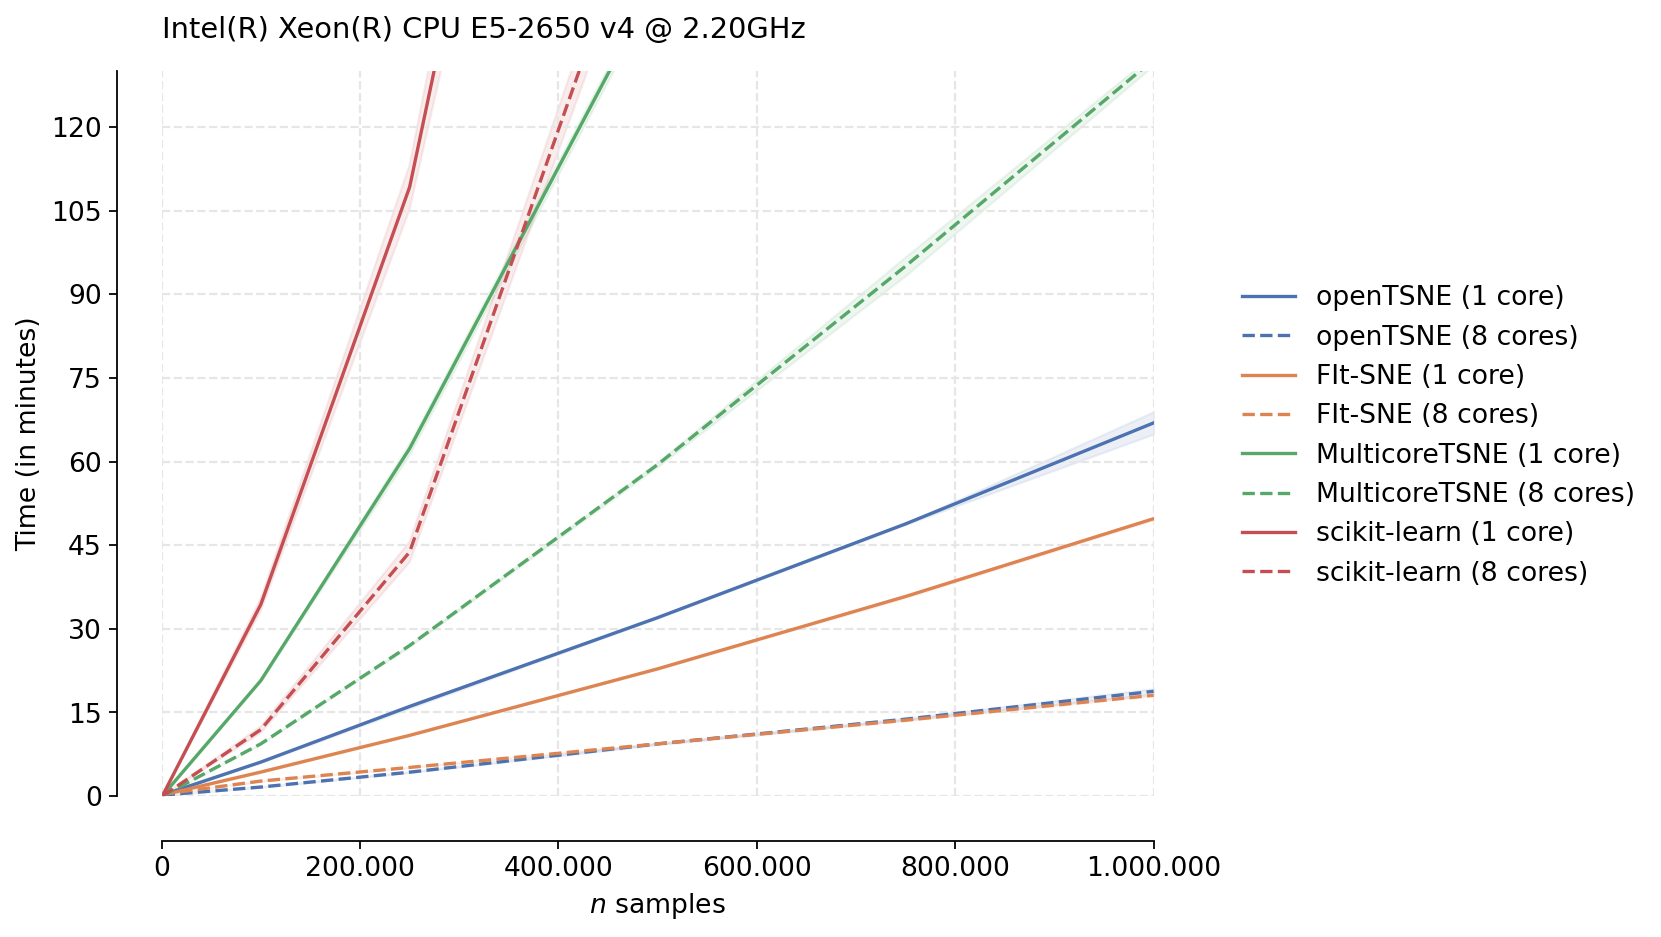
\includegraphics[width=0.8\textwidth]{figures/python_tsne_benchmarks.png}
    \caption{Benchmark of the best open-source t-SNE Python implementations by \cite{Poličar2023}. (Source: original webpage.)}
    \label{fig:python_tsne_benchmarks}
\end{figure}